\documentclass{standalone}
\usepackage[T1]{fontenc}
\usepackage[utf8]{inputenc}
\usepackage{pgf,tikz}
\usepackage{setspace}
\usepackage{pgfplots}
\pgfplotsset{compat=1.13}

\begin{document}

\def\sysCont{2*tf([1], [1, 0])*tf([2], [1, 2])*tf([3], [1, 3]);}
\def\samplePeriod{0.3}


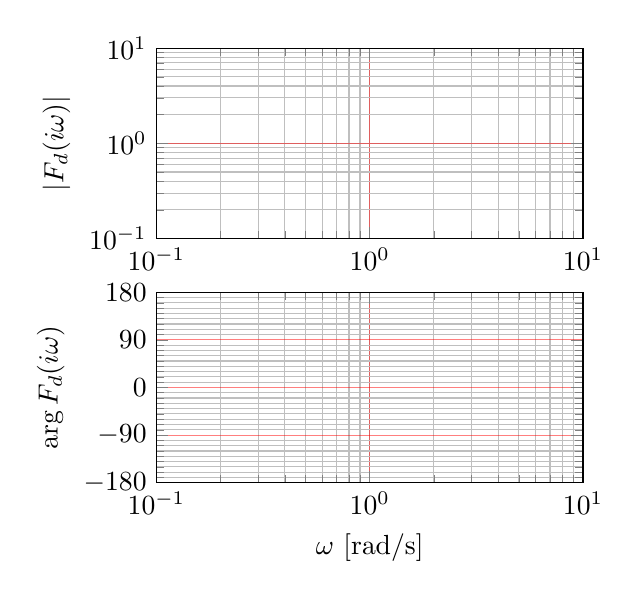
\begin{tikzpicture}
  \begin{semilogxaxis} [
      xlabel={$\omega$ [rad/s]},
      ylabel=$\arg F_d(i\omega)$,
      width=7cm,
      height=4cm,
      grid=both,
      every major grid/.style={red, opacity=0.5},
      ytick={-180, -90, 0, 90, 180},
      %yticklabels={$-45^\circ$, $0^\circ$, $45^\circ$}, 
      %xtick={0.1, 1, 10},
      %xticklabels={$0.1\omega_0$, $\omega_0$, $10\omega_0$},
      ymin=-180, ymax=180,
      xmin=0.1, xmax=10,
      minor y tick num=8,
      %legend entries={Bessel filter, Delay of one},
      %legend pos={south west},
  ]
  \end{semilogxaxis}
  \begin{loglogaxis} [
      ylabel=$|F_d(i\omega)|$,
      yshift = 3.1cm, 
      width=7cm,
      height=4cm,
      grid=both,
      every major grid/.style={red, opacity=0.5},
      %ytick={0.5, 2},
      %yticklabels={$\frac{J\omega_0}{k_d2}$, $\frac{2J\omega_0}{k_d}$},
      %xticklabel=\empty,
      ymin=0.1, ymax=10,
      xmin=0.1, xmax=10,
      %legend entries={Bessel filter, Delay of one},
      %legend pos={south west},
  ]
  \end{loglogaxis}

\end{tikzpicture}

\end{document}
